\documentclass[tikz,border=5mm]{standalone}
\usetikzlibrary{positioning}

\begin{document}

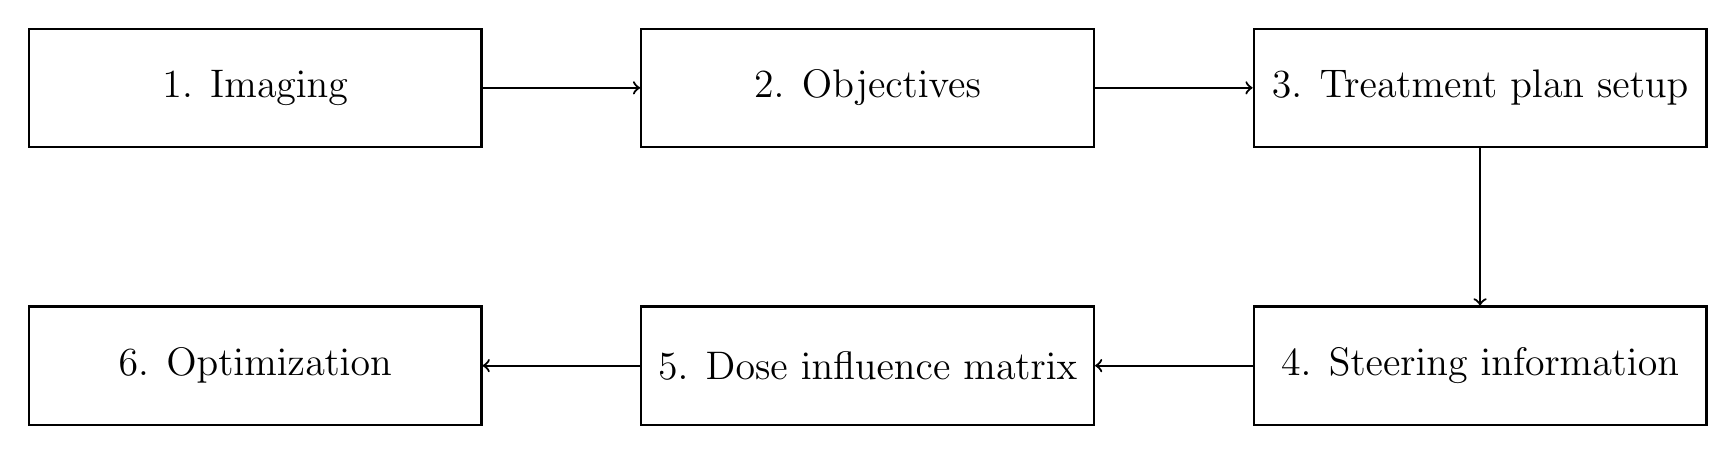
\begin{tikzpicture}[node distance=2cm, thick]
    % Define nodes with uniform size
    \node[draw, minimum width=5.75cm, minimum height=1.5cm] (A) {\Large 1. Imaging};
    \node[draw, minimum width=5.75cm, minimum height=1.5cm, right=of A] (B) {\Large 2. Objectives};
    \node[draw, minimum width=5.75cm, minimum height=1.5cm, right=of B] (C) {\Large 3. Treatment plan setup};
    \node[draw, minimum width=5.75cm, minimum height=1.5cm, below=of C] (D) {\Large 4. Steering information};
    \node[draw, minimum width=5.75cm, minimum height=1.5cm, left=of D] (E) {\Large 5. Dose influence matrix};
    \node[draw, minimum width=5.75cm, minimum height=1.5cm, left=of E] (F) {\Large 6. Optimization};

    % Draw arrows
    \draw[->] (A) -- (B);
    \draw[->] (B) -- (C);
    \draw[->] (C) -- (D);
    \draw[->] (D) -- (E);
    \draw[->] (E) -- (F);
\end{tikzpicture}

\end{document}
